ブックマークに対するGoogle ChromeのUIは非常に貧弱であり,デフォルトの状態で大量に存在するブックマークを整理する際,多くの工数がかかってしまう.
 この乱雑に増え続けるブックマークに対する効果的なアプローチは現在存在せず,ブックマークサービスとして現存するSpeed DialやBookmark Managerのようなアドオンを使うことである程度の整理することができるが,大量のブックマーク整理に向いていない.
 上記の問題を解決するべく,我々はシンプルにブックマークを管理するCloudBMを作成した.CloudBMを使うことにより,たった数回の操作で簡単に大量のブックマークを整理することが可能となる.具体的にはフォルダ分けやタグ付けを行い,さらにリンク切れをしたブックマークの削除などを自動で行い,ユーザーはただまとめられたブックマークを検索をすれば良い.
\subsection{実装した機能}
\begin{itemize}
\item ブックマークの表示
\item ブックマークの操作
\begin{itemize}
\item DnDによるブックマークのフォルダ移動
\item DnDによるブックマークの並び替え
\end{itemize}
\item ブックマークの検索とグルーピング
\begin{itemize}
\item タイトル等からの検索
\item ブックマークのページ内容による検索
\end{itemize}
\end{itemize}

\subsection{システム構成}
以下に本システムのシステム構成を示す.
\begin{figure}[htbp]
  \begin{center}
    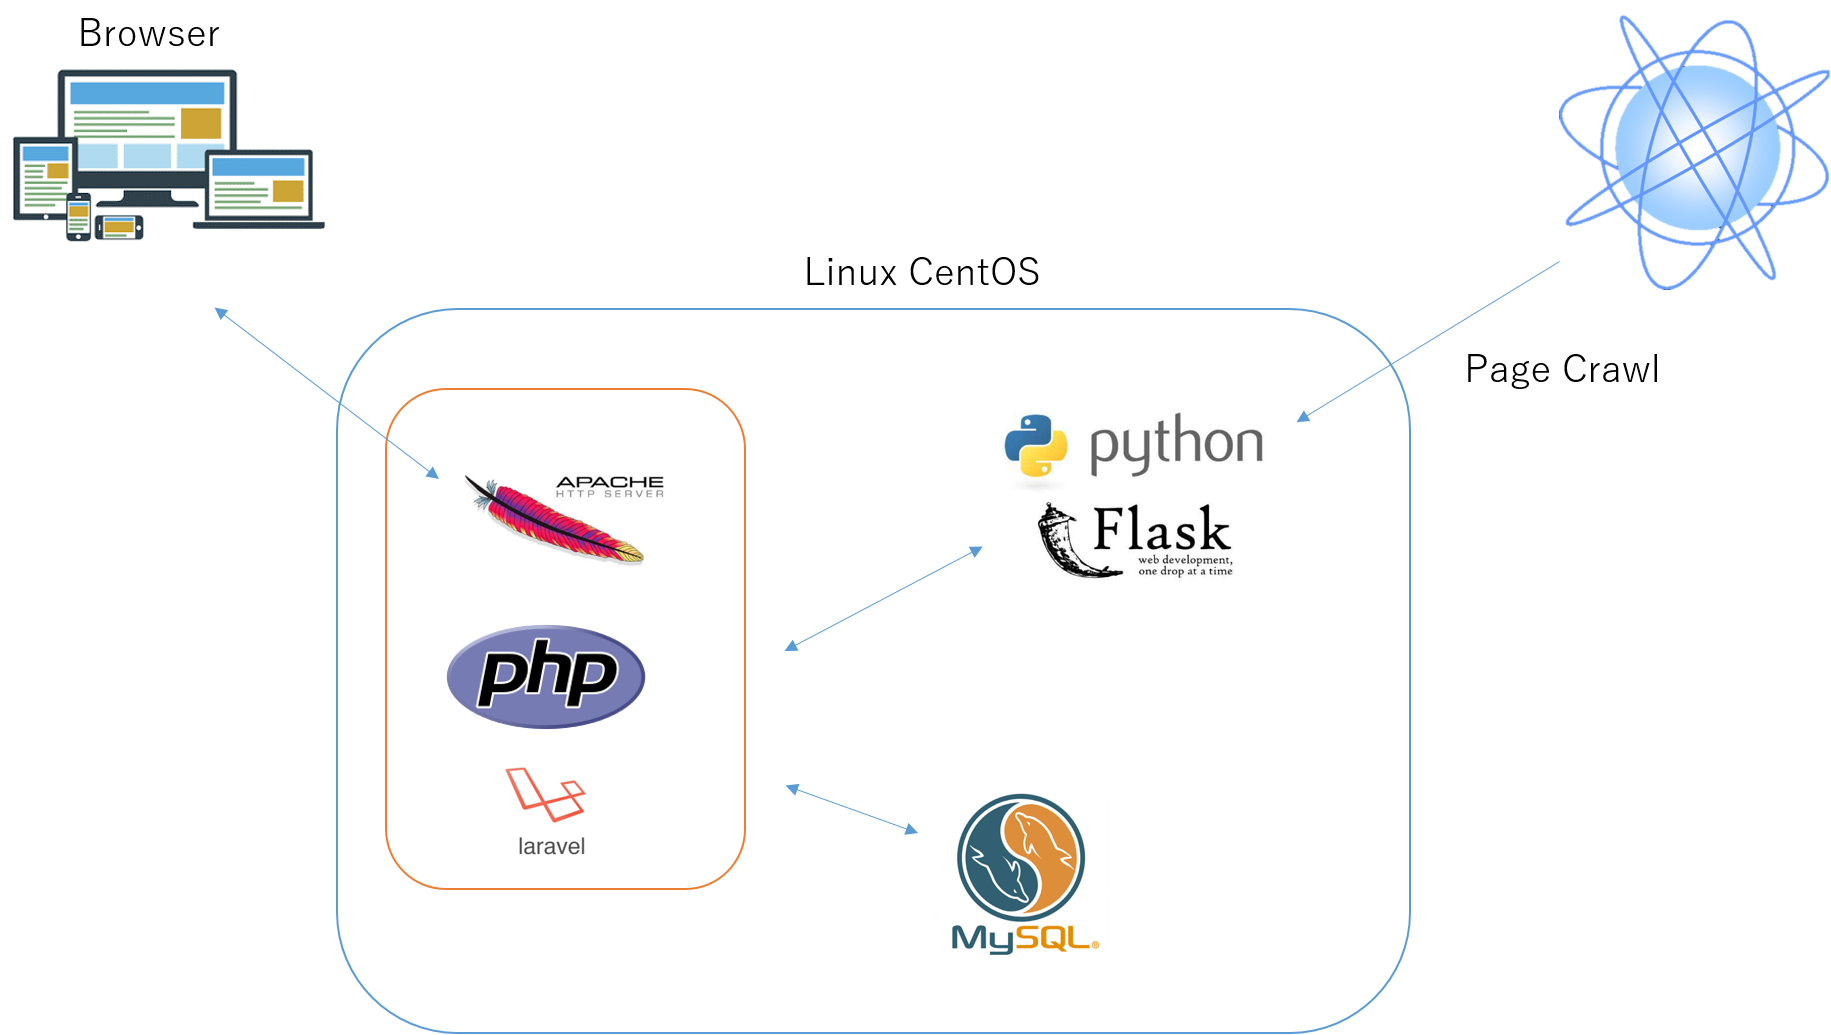
\includegraphics[clip,width=7.0cm]{./architecture.png}
    \caption{システムアーキテクチャ}
    \label{fig:system}
  \end{center}
\end{figure}
本システムはSPAとして構成する.\par
図にしめしたように,フロントサイドではJSフレームワークとしてVuejsを用いる. またサーバーとの通信に関してはAjaxを利用する.
サーバーサイドはLinux環境内にWEBサーバーとしてApacheを,データベースとしてMySQLを用意する. ApacheではPHPを利用しフロントサイドより呼び出すAPIを実装する.\par
加えてサーバーサイドではブックマークの内容解析を行うためのAPIを用意する. このAPIはpythonとpythonのWebフレームワークであるflaskで構成されておりphpから利用される.\\
\par
使用する主なソフトウェア・言語・ライブラリのバージョンについては以下の通りとする.
\begin{itemize}
 \item フロントエンド
    \begin{itemize}
    \item HTML5
    \item CSS3
      \item Bootstrap 3.6
      \item JavaScript ES5
      \item Vuejs 1.x系.
     \end{itemize}
 \item サーバサイド
     \begin{itemize}
    \item PHP 7
    \item Laravel  5.1
      \item MySQL 5.6
      \item Python 3.5
      \item Flask 0.11
     \end{itemize}
\end{itemize}
